\documentclass[conference]{IEEEtran}
\usepackage[T1]{fontenc}
\usepackage{amsmath,amssymb,amsthm}
\usepackage{graphicx,booktabs}
\usepackage[hidelinks]{hyperref}
\newtheorem{theorem}{Theorem}
\newtheorem{proposition}[theorem]{Proposition}
\newtheorem{corollary}[theorem]{Corollary}
\newcommand{\E}{\mathbb{E}}
\newcommand{\Prob}{\mathbb{P}}
\newcommand{\ind}{\mathbf{1}}
\newcommand{\simplex}{\Delta_d}
\DeclareMathOperator{\Bin}{Bin}
\DeclareMathOperator{\Hyp}{Hypergeom}
\title{Auditing Failure Across an Attack Suite under Per-Input Query Limits}
\author{Anonymous submission}
\begin{document}
\maketitle
\begin{abstract}
An audit that tests only part of an attack suite observes a detection rate, which need not reflect the probability of failure under the complete suite. This paper studies that distinction when the audit has a hard limit of k attack evaluations per input. Outcomes may have arbitrary dependence, and attack selection may be adaptive. For outcome-only auditors, an exact reduction equates the finite-sample minimax problem to estimation from hypergeometric mixture counts. An exact total-budget theorem characterizes the smallest worst-case probability of observing no failures at each fixed failure prevalence, including adaptive and randomized audits. Classical approximation duality characterizes the remaining ambiguity: with 64 attacks and a cap of four, populations with complete-suite failure rates of 100\% and 21.6\% can be observationally indistinguishable. When additional evaluations are permitted on selected inputs, a two-phase audit screens broadly and randomly completes initially undetected cases. An unbiased estimator, finite-sample confidence interval, and exact variance expression account for this selection. Evaluation on frozen security benchmarks and measured classifier matrices compares certified population ambiguity with finite-sample interval width and compares precision against both reserved budgets and actual evaluations with early stopping. Controlled low-failure experiments separate point-estimation precision from certification success. The results concern a fixed suite and a stated observation protocol, rather than security against unrestricted attacks.
\end{abstract}
\begin{IEEEkeywords}
security evaluation, attack suites, audit design, partial identification, minimax inference
\end{IEEEkeywords}

\section{Introduction}
Security evaluations use complementary attacks because different procedures expose different failures~\cite{carlini,croce}. When the target is failure under any attack in a fixed suite, a detected success establishes suite failure, whereas an unsuccessful partial search does not establish resistance to untested attacks. More inputs can estimate a partial-search detection rate precisely while leaving the complete-suite rate unidentified.

The distinction concerns the measurement protocol. If a threat model restricts an attacker to a specified budget, success within that budget is a legitimate target, as in Fair-ASR~\cite{fairasr}. Here the target is fixed across the complete suite, and the resource restriction limits its measurement. The decision is whether additional shallow screening can support complete-suite certification or the owner must authorize deeper verification. Section~\ref{sec:contract} specifies a proposed observation contract for this decision; its restrictions are not asserted to be an established operational bottleneck.

The main mathematical result compares all permitted adaptive designs under a hard per-input cap. For outcome-only auditors, whose selection decisions use attack identities and observed bits, Theorem~\ref{thm:reduction} equates finite-sample minimax risk to a hypergeometric mixture experiment without increasing the cap. Uniform subset sampling preserves the minimax value, and a parameter-independent simulation covers early stopping and interleaving. A second result concerns zero detections under a total budget. Building on the survival calculation in multi-urn search~\cite{marks}, Theorem~\ref{thm:zero-budget} gives the fixed-budget minimax value over unrestricted binary-vector populations. Completing inputs and spending the remainder on one uniform subset attains the bound; inversion calibrates a common upper endpoint after zero detections.

The reduction also obstructs certification. At $d=64,k=4$, indistinguishable populations can have failure rates of 1.293\% and 6\%. A capped gate with false-certification probability at most 5\% above a 5\% threshold must pass the low-rate population with probability at most 5\%, for every fixed sample size. Under a 12,800-evaluation ceiling, 200 complete labels support 88.1\% power (Section~\ref{sec:gate-obstruction}). This is a constructed consequence, not deployment evidence. The separate zero-detection example saves only 2.3\%; exact calibration need not give large efficiency gains.

Classical approximation duality, linear estimation, and two-phase verification~\cite{polyanskiy,wu,begg,mcnamee} supply supporting inference tools. The certification separation is a consequence of the design reduction. Frozen benchmark replay and pilot ordering illustrate differences between identification, point precision, confidence procedures, and expenditure; they do not establish an optimal ranking of audit procedures.

\section{Related Work}
\paragraph{Security evaluation across attacks}
Carlini et al.~\cite{carlini} identify failures in robustness evaluation, and AutoAttack combines complementary attacks~\cite{croce}. JailbreakBench releases standardized attack artifacts~\cite{jbb}; StrongREJECT assesses whether responses meaningfully answer harmful requests~\cite{strong}. Maple et al.~\cite{maple} explicitly advocate union coverage across configurations. The present target follows that union perspective and asks what a restricted observation protocol can identify. AutoAttack stops evaluating an input after a successful attack~\cite{autocode}. Fair-ASR measures success under shared target-call budgets and tracks attacker calls separately~\cite{fairasr}; the present unit is a completed, fixed attack procedure.

\paragraph{Population recovery}
The target is one minus the mass of the all-zero vector, as in lossy population recovery~\cite{moitra,polyanskiy}. Polyanskiy et al.~\cite[Theorem~4 and Remark~5]{polyanskiy} give finite-mixture estimation bounds and a permutation-invariance reduction. Under independent erasures, the total retained count $K$ is independent of $S$; conditional on $K=k$, retained ones follow exactly~\eqref{eq:H}. The fixed-depth channel is therefore a conditional version of that observation model. Independent erasures retain every coordinate with positive probability, whereas a cap $k<d$ excludes that event. Theorem~\ref{thm:reduction} additionally compares all permitted adaptive query designs at fixed $m,k,d$.

\paragraph{Testing distributions through coordinate queries}
Goldreich and Ron's Huge Object model~\cite{hugeobjects} samples independent binary strings and accesses them through coordinate queries, using earth mover distance induced by relative Hamming distance. For index-invariant properties, Chakraborty et al.~\cite[Theorem~F.1]{indexinvariant} convert an adaptive tester using $s$ samples and $q$ queries into a nonadaptive tester using the same samples and at most $sq\leq q^2$ queries. Adar and Fischer~\cite{adaptivity} distinguish information flow between samples and establish adaptivity separations. Those results concern property testing and query complexity. Theorem~\ref{thm:reduction} instead equates finite-sample minimax risks for the stated scalar functional and arbitrary nonnegative loss, preserving the per-input cap without query overhead.

\paragraph{Moment identification and approximation}
Matched moments and polynomial approximation provide established inference tools~\cite{wu}. Approximation of symmetric Boolean functions~\cite{paturi} gives the OR depth scale used in Section~\ref{sec:identification}. Singh and Singh~\cite{singh} characterize fixed-rollout pass@$k$ identification in a conditional-binomial model. Here the suite is finite, outcomes can be arbitrarily dependent, and sampling is without replacement. The adaptive-design comparison precedes the application of this classical identification machinery.

\paragraph{Selective verification}
Begg and Greenes~\cite{begg} analyze verification bias when follow-up depends on screening results. McNamee~\cite{mcnamee} studies two-phase prevalence estimation and case detection under a fixed budget. Section~\ref{sec:completion} specializes this structure to a one-sided attack screen: a positive outcome establishes suite failure. The resulting exact variance and stopping-cost expressions support the audit comparisons.

\paragraph{Failure discovery and test allocation}
Marks and Zaman~\cite{marks} analyze multi-urn search. For independent size-$d$ urns containing one uniformly located success with probability $\theta$, their Corollary~2 gives survival probability $\prod_i(1-\theta t_i/d)$ after $t_i$ queries to urn $i$. Their Theorems~2 and~4 establish block-policy optimality for expected search cost. Theorem~\ref{thm:zero-budget} instead minimizes worst-case miss probability at each fixed budget over unrestricted binary-vector populations. The singleton urn model is least favorable; a concentration argument handles the remainder, and uniform sampling attains the bound throughout the population class. Expected-cost optimality alone does not imply this fixed-horizon result. The confidence interpretation concerns a common nonrandom endpoint after zero detections. Partition testing~\cite{chen} addresses the different allocation of complete test cases among input subdomains.

\section{Audit Model and Security Target}\label{sec:model}
Fix a model, a failure predicate, and $d$ attack procedures. For an independently sampled input, define
\begin{equation}
 \begin{aligned}
 V&=(V_1,\ldots,V_d)\in\{0,1\}^d,\quad S=\sum_{a=1}^d V_a,\\
 \theta(P)&=\Prob_P(S>0).
 \end{aligned}
\end{equation}
Here $V_a=1$ means that attack $a$ causes the defined failure. The law $P$ of $V$ is unrestricted. In particular, the coordinates need not be independent, identically distributed, or exchangeable. The target $\theta(P)$ is \emph{complete-suite failure}. It is an empirical attack-suite target, not a guarantee over an unenumerated perturbation set or all possible attackers.

An audit has $m$ independent inputs with vectors $V^{(1)},\ldots,V^{(m)}$. It may query at most $k$ distinct coordinates of each vector, where $1\leq k\leq d$. It may use previously observed outcomes from any input when deciding which coordinate to query next. Repeated queries of a coordinate reveal the same bit and provide no additional information. Its internal randomness is independent of the inputs.

The theoretical auditor receives input indices, attack indices, and queried bits. It does not receive model scores, gradients, embeddings, readable input content, or other features informative about unqueried bits. This is an outcome-only benchmark audit. Actual attack generation can use the input; the restriction concerns the \emph{audit-selection policy} considered in the theorem. 

The fixed-vector model applies directly to deterministic attacks and a deterministic evaluated system. For randomized procedures, it applies conditionally to a prespecified set of seeded executions, provided querying one entry does not change another entry's outcome. Fresh unseeded reruns, stateful defenses, and attacks that modify subsequent procedures require a different model. A historical binary benchmark matrix is also a fixed-vector experiment, but its target is the archived outcome, not a future-response probability.

Each coordinate query is assigned unit cost and denotes one completed attack procedure. Actual model calls, tokens, and wall time can differ across procedures; the numerical budget comparisons count revealed suite outcomes. Within-attack access and search budgets are part of the fixed procedure definition.

\subsection{A proposed security-evaluation contract}\label{sec:contract}
Consider an independent audit of an agent that processes untrusted documents, with unauthorized program execution as the failure predicate. NIST's agent-hijacking evaluations include this security endpoint~\cite{nistagent}. A deployment owner registers 36 injection procedures, fixed system and grader versions, and seeded executions. A trusted service draws independent task environments from a declared distribution and restores each environment before each procedure, so one execution cannot change another's outcome.

The external statistical auditor receives record identifiers and queried bits; task content, traces, and execution privileges remain with the execution team. This permits checking the statistical rule without distributing task environments. Separately, the owner reserves an initial allowance of four procedures per record across a broad, prespecified screening cohort, so difficult cases cannot consume other records' allowances. This breadth policy serves initial failure discovery and comparison; it need not optimize suite-wide certification. AISI documents differentiated information access and evaluation tiers~\cite{aisievaluation}, but this interface and quota are proposed choices, not reported institutional practice. Restricted access does not make the quota necessary.

The owner decides whether to retain the cap or authorize confirmation under a total ceiling without per-record caps. Confirmation draws fresh records from the same registered distribution and preserves the suite and failure predicate. Earlier screening is charged separately. Each query consumes one evaluation unit; heterogeneous runtimes are not equated. The illustrative gate requires a one-sided 95\% upper bound at most 5\%, a calculation threshold rather than a proposed deployment tolerance for unauthorized execution. Section~\ref{sec:decision} derives its zero-detection budget. Honest execution and reporting are assumed. This is a design calculation, not a new agent experiment.

\subsection{Uniform subset observations}
If an audit chooses a size-$k$ subset uniformly without replacement, its count of successful attacks $C$ satisfies
\begin{equation}\label{eq:H}
 H_{cs}=\Prob(C=c\mid S=s)
 =\frac{\binom{s}{c}\binom{d-s}{k-c}}{\binom{d}{k}},
 \quad c=0,\ldots,k.
\end{equation}
An infeasible binomial coefficient is zero. Let $\mu_s=\Prob(S=s)$, let $\simplex$ be the probability simplex on $\{0,\ldots,d\}$, and set $h_s=\ind\{s>0\}$. Then
\begin{equation}\label{eq:inverse}
 q=H\mu,\qquad \theta=h^\top\mu=1-\mu_0.
\end{equation}
Equation~\eqref{eq:H} holds for every fixed vector with $s$ ones, irrespective of their locations. Therefore the count experiment remains valid even when the underlying suite is highly asymmetric.

\section{An Exact Minimax Reduction}\label{sec:reduction}
For a nonnegative loss $\ell(t,\theta)$, define the optimal risk over all permitted audit designs and randomized estimators by
\begin{equation}
 \mathcal R_{m,k,d}=\inf_{\mathcal A,\widehat\theta}
 \sup_P \E_P\ell(\widehat\theta,\theta(P)).
\end{equation}
Define the scalar-experiment risk
\begin{equation}
 \mathcal R^{H}_{m,k,d}=\inf_{\widehat t}\sup_{\mu\in\simplex}
 \E_{C_1,\ldots,C_m\sim(H\mu)^{\otimes m}}
 \ell(\widehat t,1-\mu_0).
\end{equation}
Both infima permit independent estimator randomness. The formulations have the same decision space.

\begin{theorem}[Optimal design under a hard cap]\label{thm:reduction}
For every $m,d,k$ and nonnegative loss for which these risks are defined,
\begin{equation}\label{eq:reduction}
 \mathcal R_{m,k,d}=\mathcal R^{H}_{m,k,d}.
\end{equation}
Uniform independent size-$k$ subset sampling attains the minimax value when an optimal count estimator exists, and otherwise approaches it arbitrarily closely through count estimators.
\end{theorem}
\begin{proof}
For the upper bound, run uniform subset sampling and retain its counts. By~\eqref{eq:H}, any population $P$ produces the scalar experiment for its distribution $\mu$ of $S$. Any count estimator therefore has the same risk as in that experiment. Taking the infimum gives $\mathcal R_{m,k,d}\leq\mathcal R^H_{m,k,d}$.

For the reverse inequality, restrict $P$ to the following subclass. Draw $S\sim\mu$, then place its $S$ ones uniformly among the $d$ coordinates. Inputs are independent. This constructs a legitimate population $P_\mu$ for every $\mu\in\simplex$.

On this subclass, consider any adaptive audit. After it has queried $t$ distinct coordinates on an input and seen $u$ ones, the remaining coordinates are symmetric conditional on $S$. Any new coordinate has success probability $(S-u)/(d-t)$. Which unused label is selected does not affect this probability. Thus the successive new-coordinate outcomes form a sample without replacement from $S$ ones and $d-S$ zeros, regardless of adaptive label choices.

The full interaction can be simulated from $m$ independent count observations. For each input $i$, given $C_i=c$, independently generate a uniformly random length-$k$ binary string containing $c$ ones. Supply its next unused bit whenever the audit queries a new coordinate on that input. Repeated coordinates receive their stored bit. For an ordered string $w$ with $c$ ones, its conditional probability given $S=s$ is $H_{cs}/\binom{k}{c}$. Hence conditional on $C_i$, the ordering is uniform and independent of $\mu$. Consequently the simulation uses a parameter-independent randomization. It remains valid if the audit stops early or interleaves different inputs, because the streams can be generated before any interaction.

Every adaptive estimator on the subclass is therefore implementable from the count experiment, with the same distribution and risk. Its worst-case risk over all $P$ is at least the optimal count risk over $\mu$. Taking infima proves the reverse inequality.
\end{proof}

The theorem concerns unrestricted minimax risk, not sufficiency for each nonsymmetric population: a dominant attack can be worth prioritizing. Symmetric populations supply the lower bound, while uniform sampling works throughout the class. The result compares designs without giving a closed-form finite-sample minimax estimator.

\section{Identification and Inference under a Cap}\label{sec:identification}
\subsection{Population identification}
Suppose the count law $q$ is known exactly. This is an optimistic population limit, with no sampling error. Its identified interval is
\begin{equation}\label{eq:identified}
 I(q)=\left[\min_{\mu\in\simplex:H\mu=q}h^\top\mu,
              \max_{\mu\in\simplex:H\mu=q}h^\top\mu\right].
\end{equation}
The finite-dimensional feasible set is compact and convex, so the endpoints exist and every intermediate value is attainable. An individual $I(q)$ can be a singleton even when $k<d$. The worst-case width is
\begin{equation}\label{eq:D}
 D_{k,d}=\max_{\mu,\nu\in\simplex:H\mu=H\nu}
 \left|h^\top(\mu-\nu)\right|.
\end{equation}

\begin{proposition}[Observable polynomials]\label{prop:moments}
Two distributions $\mu,\nu$ have the same count law if and only if they agree on expectations of all polynomials in $S$ of degree at most $k$.
\end{proposition}
\begin{proof}
Writing $(z)_j=z(z-1)\cdots(z-j+1)$, sampling without replacement gives
\begin{equation}\label{eq:factorial}
 \E[(C)_j]=\frac{(k)_j}{(d)_j}\E[(S)_j],\quad 0\leq j\leq k.
\end{equation}
For example, both sides count ordered $j$-tuples of successful queried coordinates. The falling factorials form a polynomial basis. Conversely, each $H_{cs}$ in~\eqref{eq:H}, interpreted as a polynomial in $s$, has degree at most $k$, so matched polynomial expectations determine the count probabilities.
\end{proof}

\begin{theorem}[Exact worst-case ambiguity]\label{thm:diameter}
Let $\mathcal P_k$ denote univariate polynomials of degree at most $k$. Then
\begin{equation}\label{eq:approx}
 D_{k,d}=2\min_{p\in\mathcal P_k}\max_{s\in\{0,\ldots,d\}}
             |h_s-p(s)|.
\end{equation}
For squared loss, every capped audit has worst-case risk at least $D_{k,d}^2/4$, for every $m$.
\end{theorem}
\begin{proof}
If $H\mu=H\nu$, Proposition~\ref{prop:moments} implies that the expectation of any $p\in\mathcal P_k$ cancels. Therefore
\[
 |h^\top(\mu-\nu)|\leq 2\max_s|h_s-p(s)|.
\]
If the optimal approximation error $e$ is zero, the upper bound already proves the assertion. Assume $e>0$. For equality, finite linear-programming duality for uniform approximation gives a signed vector $z$ with $\|z\|_1=1$, orthogonal to every degree-$k$ polynomial, whose pairing with $h$ equals $e$; the positive optimum saturates the dual constraint $\|z\|_1\leq1$. Orthogonality to the constant implies that the positive and negative parts each have mass $1/2$. Thus $\mu=2z_+$ and $\nu=2z_-$ are probability laws, have the same count law, and have target separation $2e$. This applies standard approximation--moment duality to the finite observation operator~\cite{wu}.

By the simulation in Theorem~\ref{thm:reduction}, the symmetric vector populations corresponding to an extremizing pair are indistinguishable under every capped audit. If their target values are $a,b$, the estimator has a common distribution $Z$ in both populations. The average squared error satisfies
\[
 \tfrac12\E[(Z-a)^2+(Z-b)^2]
 =\E[(Z-(a+b)/2)^2]+(a-b)^2/4.
\]
The larger risk is at least this average and hence at least $D_{k,d}^2/4$.
\end{proof}

For interpretation, a symmetric multivariate polynomial approximating OR on $\{0,1\}^d$ reduces to a univariate polynomial in the Hamming weight $s$. Conversely, a degree-$k$ polynomial in $s=\sum_a V_a$ gives a degree-at-most-$k$ polynomial on the cube. Thus~\eqref{eq:approx} is precisely the established approximate-degree problem for OR. Paturi's result~\cite{paturi} implies that reducing worst-case width below a fixed nontrivial constant requires and permits $k$ of order $\sqrt d$, with constants depending on the requested width. This is an identification statement with the count law known; it does not promise that a practical number of inputs estimates that law accurately enough.

For $d\geq2$, simple exact values check the formulation:
\begin{equation}\label{eq:checkpoints}
 D_{1,d}=1-1/d,\qquad D_{d-1,d}=2^{1-d},\qquad D_{d,d}=0.
\end{equation}
The elementary constructions for these checks are given in Appendix~\ref{app:checks}.

\subsubsection{Exact computational witnesses}
All population programs in this paper use the actual finite support $\{0,\ldots,d\}$; there is no continuous-support discretization. Numerical linear programming first identifies candidate extremal supports. Rational interpolation and rational probability weights then verify matched moments, normalization, target separation, and the dual polynomial inequality at \emph{every} support point.

The sweep covers $d\in\{16,32,64,128\}$ and admissible $k\in\{1,2,4,8,16,32\}$. All 23 settings were executed and certified, including full-suite cases. Figure~\ref{fig:diameter} shows all settings. For $d=64,k=4$, the exact targets are 1 and $512/2375$; their gap is $1863/2375$. These populations also have identical \emph{labeled adaptive transcripts}, when lifted through the symmetric construction. The uncertainty is consequently not an artifact of discarding attack labels after collection. Mixing both with an all-zero vector with probability $1-\lambda$ preserves indistinguishability and scales both failure probabilities by $\lambda$. Section~\ref{sec:gate-obstruction} uses this fact for a certification decision.


\begin{figure}[t]
\centering
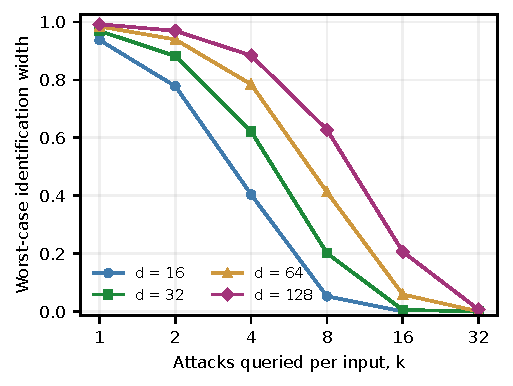
\includegraphics[width=\columnwidth]{figures/diameter.pdf}
\caption{Worst-case target ambiguity under the per-input cap. Values come from finite programs with rational certificates. Smaller width at larger depth concerns population identification; finite-sample precision is a separate requirement.}\label{fig:diameter}
\end{figure}

\subsection{Confidence intervals from partial observations}\label{sec:confidence}
A finite audit observes a histogram $n_0,\ldots,n_k$ from $m$ independent uniformly sampled subsets. Substituting the empirical histogram directly into~\eqref{eq:identified} is unsafe: it may not lie in the image of any hypergeometric mixture and has sampling error even when it does. Instead, construct a simultaneous confidence region for $q$ and project it through the finite inverse problem.

For $x$ successes out of $m$ trials, let $\operatorname{CP}_\alpha(x,m)$ denote the two-sided Clopper--Pearson interval with noncoverage at most $\alpha$~\cite{clopper}. 

For $k<d$, the implementation spends half the error budget on the categories and half on the overall detection rate:
\begin{align}
 [l_c,u_c]&=\operatorname{CP}_{\delta/[2(k+1)]}(n_c,m),\\
 [l_D,u_D]&=\operatorname{CP}_{\delta/2}(m-n_0,m).
\end{align}
Define
\begin{equation}\label{eq:confset}
 \mathcal C=\left\{\mu\in\simplex:
 \begin{array}{l}l_c\leq (H\mu)_c\leq u_c\ \ \forall c,\\
 l_D\leq1-(H\mu)_0\leq u_D
 \end{array}\right\}.
\end{equation}
Report the minimum and maximum of $h^\top\mu$ over $\mathcal C$. If the set is empty, report $[0,1]$ and flag the inconsistency. When $k=d$, use $\operatorname{CP}_\delta(m-n_0,m)$ directly.

\begin{proposition}[Finite-sample coverage]\label{prop:coverage}
Under uniform subset sampling and the model of Section~\ref{sec:model}, the projected interval contains $\theta(P)$ with probability at least $1-\delta$ for every population $P$.
\end{proposition}
\begin{proof}
Each category count has a binomial marginal, even though the histogram entries are dependent. A union bound over category noncoverage gives probability at most $\delta/2$. The detection interval adds at most $\delta/2$. On the complementary event the true $\mu$ satisfies every constraint in~\eqref{eq:confset}, so its target belongs to the projected range. The fallback cannot reduce coverage. The full-suite case is the usual binomial interval.
\end{proof}

This construction is deliberately conservative and is not asserted to be the finite-sample minimax estimator. It uses $d+1$ nonnegative variables and two linear objectives. The guarantee applies to the stated randomized sampling protocol, not automatically to histograms retained by an arbitrary adaptive collection policy.

A useful baseline retains only whether the partial audit detected anything. Let $a=\Prob(C>0)$. Given $S>0$, uniform sampling detects at least one success with probability between $k/d$ and 1. Hence
\begin{equation}\label{eq:detector}
 a\leq\theta\leq\min(1,da/k).
\end{equation}
Both endpoints are attainable for suitable mixtures, so this is sharp given only $a$. Substituting a $1-\delta$ binomial interval for $a$ gives a valid detection-only interval. The full-count projection can use overlap information absent from this baseline, but the split error budget means finite-sample domination is not guaranteed in every sample.

The implementation uses double-precision beta quantiles, conservatively repaired LP dual multipliers, and an outward allowance. Mathematical coverage is distinct from formal numerical certification: beta-quantile inversion is not checked by interval arithmetic. Population witnesses are separately verified using exact fractions.

\subsection{An explicit estimator and finite-sample risk}
For a classical linear-estimation baseline~\cite{polyanskiy}, fix $g\in\mathbb R^{k+1}$ before the audit and define
\begin{equation}
 \beta_g=\|H^\top g-h\|_\infty,\qquad
 G_g=\max_c g_c-\min_c g_c.
\end{equation}
For $\widehat\theta_g=m^{-1}\sum_i g_{C_i}$, the bias is at most $\beta_g$, and bounded-variable variance gives
\begin{equation}\label{eq:linear-risk}
 \sup_\mu\E_\mu(\widehat\theta_g-\theta)^2
 \leq \beta_g^2+G_g^2/(4m).
\end{equation}
The implementation minimizes $\beta_g+G_g/(2\sqrt m)$ by a finite linear program. This computable upper-bound criterion does not establish exact minimaxity. Clipping to $[0,1]$ cannot increase squared error. Hoeffding's inequality yields an interval centered at the untruncated estimate, with radius
\begin{equation}\label{eq:linear-ci}
 \beta_g+G_g\sqrt{\log(2/\delta)/(2m)}
\end{equation}
that contains $\theta$ with probability at least $1-\delta$. Endpoint clipping preserves coverage. This baseline and projection use the same counts; neither is assumed to dominate.

The same argument closes the asymptotic risk statement. Every degree-$k$ polynomial on the support is in the row span of $H$, so a best approximating polynomial has the form $H^\top g_*$ for some finite vector $g_*$. Its bias bound is $D_{k,d}/2$. Combining~\eqref{eq:linear-risk} with Theorem~\ref{thm:diameter} gives, for fixed $d,k$ under squared loss,
\begin{equation}
 \lim_{m\to\infty}\mathcal R_{m,k,d}=D_{k,d}^2/4.
\end{equation}
This consequence uses the established linear-estimation method. The finite-sample rate at a particular budget still depends on the variance needed to approximate the unobserved target.

\section{Allocation and Certification}\label{sec:budget}
\subsection{Complete labels under the same budget}
A hard cap is stronger than a bound on total evaluations. Suppose $mk$ coordinate evaluations are available. Independently of outcomes, select $r=\lfloor mk/d\rfloor$ inputs from the available independent input stream and determine $Y_i=\ind\{S_i>0\}$ on each. Query until the first success or suite exhaustion; this requires at most $d$ evaluations per input. For $r\geq1$, let $\widehat\theta_{\rm full}=r^{-1}\sum_iY_i$.

\begin{corollary}[An allocation consequence]\label{thm:budget}
The full-suite estimator uses at most $mk$ evaluations and satisfies
\begin{equation}\label{eq:fullmse}
 \sup_P\E_P(\widehat\theta_{\rm full}-\theta(P))^2
 \leq\frac{1}{4r}.
\end{equation}
If $D_{k,d}>0$ and $r>D_{k,d}^{-2}$, this upper bound is strictly smaller than the worst-case mean squared error of every audit with the original cap $k$ and $m$ inputs.
\end{corollary}
\begin{proof}
The $Y_i$ are independent Bernoulli observations with parameter $\theta(P)$. The estimator is unbiased and has variance $\theta(P)(1-\theta(P))/r\leq1/(4r)$. The cost is at most $rd\leq mk$. Compare this upper bound to Theorem~\ref{thm:diameter}'s lower bound $D_{k,d}^2/4$.
\end{proof}

The bound compares worst-case squared error under different allocation constraints. It is a sufficient comparison, not an optimality result among all total-budget designs or a claim of pointwise dominance. For this unweighted full-label estimator, inputs are selected independently of outcomes. Outcome-dependent completion is possible, but requires an estimator that accounts for the selection, as developed next.

The ceiling $rd$ is a reserved budget, not necessarily the number of evaluations spent. For a uniformly random attack order, let $T$ be the first successful position, with $T=d$ when all attacks fail. Conditional on $S=s$,
\begin{equation}\label{eq:fullcost}
 \E[T\mid S=s]=
 \begin{cases}d,&s=0,\\(d+1)/(s+1),&s>0.\end{cases}
\end{equation}
For $s>0$, the $s$ successful positions divide the failures into $s+1$ exchangeable gaps, giving the expression. Stopping after success, as in established attack-suite evaluation~\cite{autocode}, determines the same $Y$ at lower expected cost. Every complete-label comparator uses this rule.

\subsubsection{A certification obstruction from indistinguishability}\label{sec:gate-obstruction}
Consider any possibly randomized pass decision satisfying
\begin{equation}\label{eq:valid-gate}
 \sup_{P:\theta(P)>\tau}\Prob_{P,\mathcal A}(\mathrm{pass})\leq\delta.
\end{equation}
Let $P_-$ and $P_+$ be symmetric lifts of count laws with $H\mu_-=H\mu_+$ and $\theta_-<\tau<\theta_+$. The simulator in Theorem~\ref{thm:reduction} gives identical complete transcript distributions under these populations. Thus every capped audit satisfying~\eqref{eq:valid-gate} has $\Prob_{P_-,\mathcal A}(\mathrm{pass})\leq\delta$, for every fixed $m$, including adaptive policies. This consequence does not depend on the confidence construction.

Retain each $d=64,k=4$ witness population with probability $\lambda=3/50$, and otherwise use the all-zero vector. The targets become $\theta_-=768/59375\approx.0129347$ and $\theta_+=.06$. At $\tau=\delta=.05$, no valid cap-four gate passes this particular low-rate population with probability above 5\%. Under a matched ceiling $B=12{,}800$, cap-four sampling can query 3,200 inputs, whereas complete labeling can examine 200. For the latter, let $X$ count positive labels and pass when $X\leq4$. At the boundary,
\[
 \Prob_{\Bin(200,.05)}(X\leq4)=.0264468<.05;
\]
monotonicity makes the gate uniformly valid above the threshold. Its exact pass probability at $\theta_-$ is .8805594, or 88.1\%. Fractions verify the mixed witness and binomial probabilities in the artifact.

This constructed separation compares reserved ceilings and assigns no separate cost to acquiring inputs. For this pair, additional shallow screens cannot repair the acceptance decision; complete labels change what can be learned while preserving the suite and target. The example neither predicts deployment power nor proves optimality of the full-label gate. That gate accepts up to four failures, whereas Section~\ref{sec:zero} concerns \emph{zero-detection} endpoints.

\subsection{Screening with randomized completion}\label{sec:completion}
When selected inputs may exceed the initial cap, a two-phase audit uses partial results to decide where further verification is needed. Fix integers $m\geq1$, $1\leq k<d$, and $1\leq R\leq m$ before observing outcomes. Independently order the attacks uniformly for each of $m$ independent input records. Screen its first $k$ positions, stopping at the first success. Let $D_i$ indicate whether screening detected failure, $N=\sum_iD_i$, and $M=m-N$.

A positive screen already establishes $Y_i=1$. Select $r=\min(R,M)$ negative screens uniformly without replacement, using fresh randomness independent of their unobserved outcomes. On each selected record, continue the remaining attack order until success or exhaustion. Let $X$ be the number of selected records on which a failure is then found. This procedure uses at most
\begin{equation}\label{eq:completion-budget}
 B_{\max}=mk+R(d-k)
\end{equation}
attack evaluations. Screening may stop early because this design uses only $D_i$; the full-count projection in Section~\ref{sec:confidence} requires all $k$ outcomes.

Write $a=\Prob(D=1)$ and $b=\Prob(Y=1\mid D=0)$, taking $b=0$ when $a=1$. Then $\theta=a+(1-a)b$. Define
\begin{equation}\label{eq:completion-estimate}
 \widehat\theta_{\rm two}=
 \begin{cases}
 N/m+(M/m)(X/r),&M>0,\\
 1,&M=0.
 \end{cases}
\end{equation}
The prevalence of failure among completed negative screens estimates $b$, not $\theta$; the weights in~\eqref{eq:completion-estimate} account for their deliberate selection.

\begin{theorem}[Random completion after a one-sided screen]\label{thm:completion}
The estimator~\eqref{eq:completion-estimate} is unbiased for $\theta$. Its exact variance is
\begin{equation}\label{eq:completion-variance}
 \begin{aligned}
 \operatorname{Var}(\widehat\theta_{\rm two})
 &=\frac{\theta(1-\theta)}{m}\\
 &\quad+\frac{b(1-b)}{m^2R}
   \E\!\left[M(M-R)\ind\{M>R\}\right],
 \end{aligned}
\end{equation}
where $M\sim\Bin(m,1-a)$. For $R<m$, let
\begin{align}
 [a_L,a_U]&=\operatorname{CP}_{\delta/2}(N,m),\\
 [b_L,b_U]&=\operatorname{CP}_{\delta/2}(X,r),
\end{align}
with $\operatorname{CP}_{\alpha}(0,0)=[0,1]$. Then
\begin{equation}\label{eq:completion-ci}
 \left[a_L+(1-a_L)b_L,\ a_U+(1-a_U)b_U\right]
\end{equation}
contains $\theta$ with probability at least $1-\delta$.
\end{theorem}
Appendix~\ref{app:completion-proof} proves the statement by conditional sampling and a union bound.

If $R=m$ was fixed in advance, every full-suite label is known and a single interval $\operatorname{CP}_\delta(N+X,m)$ is used. If $R<m$ but the realized $M\leq R$, the two-component interval is retained: choosing a different interval solely on that outcome-dependent event would require a separate coverage argument. Values $R>m$ are equivalent to $R=m$ and are clipped before budgeting.

This procedure removes the asymptotic information floor when both screening and completion sample sizes grow in a fixed nonzero proportion. It can nevertheless have worse finite-budget precision than completing fewer inputs directly. Equation~\eqref{eq:completion-variance} identifies the residual verification term, which depends on hidden failure among negative screens. All allocations in the experiment are specified independently of the current audit outcomes; the exact variance is used for evaluation, not for choosing an oracle allocation after seeing the population.

The actual expenditure can be much lower than~\eqref{eq:completion-budget}. Appendix~\ref{app:cost} gives its expectation under random ordering. Actual evaluations and the reserved ceiling are reported separately, with no reinvestment of saved evaluations into an outcome-dependent sample size.

\subsection{Certification after zero detections}\label{sec:zero}
The global squared-error criterion does not resolve every security decision. Consider an audit that detects no failures and asks for a one-sided upper bound on complete-suite prevalence. If every vulnerable input has exactly one successful attack, uniform size-$k$ screening detects that failure with probability $k/d$. More generally, $a\geq\theta k/d$. Consequently
\begin{equation}
 \Prob(N=0)=(1-a)^m\leq(1-\theta k/d)^m.
\end{equation}
Equality is attainable with $\mu_0=1-\theta$ and $\mu_1=\theta$. Inverting this event gives the sharp nonrandom $1-\delta$ upper bound assigned to zero detections under uniform screening
\begin{equation}\label{eq:zero-partial}
 U_{\rm partial}=\min\{1,(d/k)(1-\delta^{1/m})\}.
\end{equation}
It can be completed into a valid confidence procedure by reporting $[0,1]$ after any positive detection. The implementation uses the corresponding one-sided binomial bound for general counts.

The cap-free total-budget problem retains the independent stream and outcome-only interface. The singleton lower-bound model is independent multi-urn search~\cite{marks}; its survival calculation and reduction to the unsuccessful query sequence are established. The following result uses them for fixed-budget minimax calibration over the larger population class.

\begin{theorem}[Zero detections under a total budget]\label{thm:zero-budget}
Fix integers $d\geq1$ and $B\geq0$, and allow audits on an unlimited independent input stream to use at most $B$ unit-cost coordinate queries. Audits may randomize, adapt, interleave inputs, and stop early. Let $E_0$ mean that no queried bit equals one. Write $B=rd+\rho$, where $0\leq \rho<d$. For every $\theta\in[0,1]$,
\begin{equation}\label{eq:zero-minimax}
 \inf_{\mathcal A}\sup_{P:\theta(P)=\theta}
 \Prob_{P,\mathcal A}(E_0)
 =L_{B,d}(\theta):=(1-\theta)^r(1-\theta \rho/d).
\end{equation}
One design attains this value for every $\theta$: determine $r$ complete-suite labels and, if $\rho>0$, query a uniform size-$\rho$ subset on one further independent input. Stopping the entire audit after any success is permitted.
\end{theorem}
\begin{proof}
For the lower bound, let a vector be all zero with probability $1-\theta$ and contain one uniformly located success otherwise. Condition on the audit's internal randomness. Its coordinate sets along the all-zero transcript are then fixed. Write $t_i\in\{0,\ldots,d\}$ for their distinct-coordinate counts, with $\sum_i t_i\leq B$. Independence gives
\[
 \Prob(E_0\mid\text{internal randomness})
 =\prod_i(1-\theta t_i/d).
\]
Repeated queries do not change this product. Concentrating two partial depths $x,y$ into $\min(d,x+y)$ and $\max(0,x+y-d)$ cannot increase it. If $x+y\leq d$, the original pair's product minus the concentrated pair's product is $\theta^2xy/d^2\geq0$. If $x+y>d$, the difference is $\theta^2(d-x)(d-y)/d^2\geq0$. Adding queries cannot increase the product either. Fill unused budget on fresh inputs and concentrate the depths until $r$ equal $d$ and one equals $\rho$. The resulting product is $L_{B,d}(\theta)$, proving the lower bound also after averaging over the internal randomness.

For the proposed design, all $r$ complete labels are negative with probability $(1-\theta)^r$. On a vulnerable additional input, uniform size-$\rho$ sampling detects success with probability at least $\rho/d$. Independence gives a no-detection probability at most $L_{B,d}(\theta)$, with equality for the singleton population.
\end{proof}

For $0<\delta<1$, define the common endpoint
\begin{equation}\label{eq:zero-optimal-bound}
 U^*_{B,d}=\sup\{\theta\in[0,1]:L_{B,d}(\theta)\geq\delta\}.
\end{equation}
For the attaining design, report $[0,U^*_{B,d}]$ on $E_0$ and $[0,1]$ otherwise. If $\theta>U^*_{B,d}$, noncoverage is at most $L_{B,d}(\theta)<\delta$; all other target values are always covered. This endpoint is sharp among valid procedures assigning one common nonrandom upper endpoint to every zero-detection transcript, including all internal seeds. If a smaller $u$ were used, choose $u<\theta<U^*_{B,d}$. The singleton population has $\Prob(E_0)\geq L_{B,d}(\theta)>\delta$ under every audit, violating coverage. The case $B=0$ also follows directly since no data are obtained.

At $B=0$, $U^*=1$; for $0<B<d$, it equals $\min\{1,d(1-\delta)/B\}$. For $B=rd>0$, it is the usual full-label zero-failure bound $1-\delta^{1/r}$. In the remaining cases $r\geq1,\rho>0$, it is the unique root of $L_{B,d}(\theta)=\delta$. These conventions include $\theta=0$ and $\theta=1$ without a limiting argument. Inverting $L_{B,d}$ is valid for the attaining design; another audit cannot use that endpoint solely because its ceiling is $B$. The theorem does not optimize general confidence procedures, squared error, or expected expenditure.

For fixed $d,k,\delta$ with $B=mk$ divisible by $d$, both~\eqref{eq:zero-partial} and~\eqref{eq:zero-optimal-bound} have leading term
\begin{equation}\label{eq:zero-rate}
 d\log(1/\delta)/B\qquad(B\to\infty).
\end{equation}
For $d=64,k=4,m=500,\delta=.05$, the partial endpoint is 9.56\%. Completing 31 inputs uses 1,984 evaluations and gives 9.21\%; allocating the remaining 16 evaluations to one fresh input gives the sharp 9.14\% endpoint. Thus a large worst-case estimation gap can coexist with similar zero-detection certification precision. The artifact checks 160 small allocation/Bellman cases using exact fractions and brackets the displayed endpoint by rational bisection. These checks support the proof; they do not replace its treatment of arbitrary policies.

\subsubsection{Budget for the proposed acceptance gate}\label{sec:decision}
For the contract in Section~\ref{sec:contract}, set $d=36$, threshold $\tau=.05$, and noncoverage $\delta=.05$. Earlier exploratory screening is charged separately. The smallest confirmatory-stage ceiling with $U^*_{B,36}\leq\tau$ is
\[
 B=2103=58(36)+15.
\]
The attaining allocation completes 58 fresh records and queries 15 uniform coordinates of another. Its worst-case zero-detection probability at $\theta=\tau$ is .0499834; at $B=2102$ it is .0500543. Monotonicity therefore establishes the integer budget threshold for the common endpoint. At the preceding budget, continuity also gives some $\theta>.05$ with zero-detection probability above .05, excluding a uniformly valid common endpoint at most .05. After zero detections, report $[0,U^*]$ with $U^*\approx .0499946$ and pass the gate; otherwise report $[0,1]$ and withhold this certificate. For every $\theta>\tau$, the probability of incorrectly passing is below .05.

Complete-label testing requires 59 records and 2,124 evaluations; uniform four-procedure screening requires 538 records and 2,152 evaluations. The saving over this screen is 49 outcomes, or 2.3\%. Thus sharp zero-detection calibration gives a smaller advantage here than the global estimation comparison. Exact fractions verify the threshold crossings and endpoint.

\section{Empirical Evaluation}\label{sec:experiments}
The evaluation asks three questions: how much ambiguity remains when the population count law is known; how finite-sample inference compares with that ambiguity; and how allocation changes estimation, certification, and actual expenditure. All security outcomes are frozen published results. The classifier matrices were measured locally. Audit simulations add sampling randomness, not new language-model responses or judgments.

\subsection{Outcome populations and audit protocol}
The StrongREJECT release~\cite{strong,strongdata} contains 47,576 evaluations: 313 contexts, 38 configurations, and four target models. Excluding the untransformed \texttt{none} baseline and, following the upstream analysis, \texttt{evil\_system\_prompt}, leaves a complete $313\times36$ matrix for each model. No entries are imputed. The failure predicate is a released score of at least 0.5. This is an operational threshold on a judge score, not a calibrated probability or an independently verified label. The release records GPT-4o-mini as judge for 47,530 evaluations and GPT-3.5-turbo for 46. Score-only derivatives and sensitivities at thresholds 0.25 and 0.75 are retained in the artifact.

The classifier study uses the scikit-learn handwritten digits dataset~\cite{sklearn,digits}. A fixed train/test split and untuned logistic regression and random forest models give 694 and 701 clean-correct eligible test images. The suite comprises 98 transformations: every position of a $2\times2$ patch set to either zero or one. A transformed prediction differing from the dataset label is a failure. These patches can change digit identity, so the results describe a wrong-label stress test rather than label-preserving adversarial robustness. Appendix~\ref{app:data} gives model and split details. Table~\ref{tab:populations} summarizes six populations, not six independent domains: four share security contexts and two share the digits dataset. A smaller label-only JailbreakBench case study~\cite{jbb,artifacts} is retained in Appendix~\ref{app:jbb}.

\begin{table}[t]
\caption{Primary frozen outcome populations. $n$ is the number of source rows; audit records are sampled with replacement. $a_k$ is the exact expected uniform-subset detection rate.}\label{tab:populations}
\centering
\begin{tabular}{lrrrrr}
\toprule
Population&$d$&$n$&$\theta$&$a_4$&$a_{16}$\\
\midrule
Dolphin&36&313&1.0000&.9039&.9988\\
GPT-3.5&36&313&.9968&.7696&.9887\\
GPT-4o-mini&36&313&.9904&.5193&.9061\\
Llama-3.1&36&313&.9904&.5496&.9327\\
Logistic&98&694&.9280&.2713&.6040\\
Forest&98&701&.7903&.1590&.4106\\
\bottomrule
\end{tabular}
\end{table}

Each empirical population is uniform over its retained rows. A hypothetical audit draws independent records with replacement. Counts follow the exact hypergeometric law conditional on the measured $S$; first-success positions follow the corresponding uniform-order law. This reproduces uniform subset and ordering experiments without assumptions on attack dependence. Repeated draws are not linked by input identity and reveal no extra source data. Costs count replayed suite evaluations, not new paid API calls, tokens, or runtime. Historical target names identify archived matrices, not current deployed-model vulnerability.

\begin{table}[t]
\caption{Overlap among successful attacks. Singleton fraction, median, and mean condition on $S>0$. Miss is the exact percentage of such inputs missed by a uniform four-attack screen.}\label{tab:overlap}
\centering
\begin{tabular}{lrrrr}
\toprule
Population&Singleton \%&Median&Mean&Miss \%\\
\midrule
Dolphin&0.00&17&16.95&9.61\\
GPT-3.5&0.32&12&11.60&22.79\\
GPT-4o-mini&5.81&6&6.55&47.57\\
Llama-3.1&3.23&7&6.84&44.51\\
Logistic&7.92&6&9.18&70.77\\
Forest&22.38&4&5.84&79.88\\
\bottomrule
\end{tabular}
\end{table}

Table~\ref{tab:overlap} makes the dependence patterns visible. A positive input with small $S/d$ is easily missed by shallow screening and takes longer to label under a uniform order. Forest has 22.38\% singleton positives, compared with 5.81\% for GPT-4o-mini; their $k=4$ conditional miss probabilities are .7988 and .4757. Their larger-suite and zero-mass differences also matter: expected full-label costs are 39.97 and 6.79 evaluations per input. After a negative screen, residual failure $b=(\theta-a)/(1-a)$ is .7506 for Forest but .9801 for GPT-4o-mini. Hence screening miss probability alone cannot predict completion variance: equation~\eqref{eq:completion-variance} also depends on $b(1-b)$ and how many negative screens are left unverified. The full conditional count distributions, including their tails, are retained in the artifact.

\subsection{Population ambiguity versus finite-sample width}
The complete matrices determine $\mu$ and hence the oracle law $H\mu$. Solving~\eqref{eq:identified} isolates population ambiguity, conditional on this empirical reference. Floating-point optimization proposes certificates; rational polynomials are then checked at every integer $s\in\{0,\ldots,d\}$. Lower and upper polynomial envelopes give rigorous outer endpoints. Where rational feasible distributions attain those endpoints to tolerance, the width is certified sharp to that tolerance. Table~\ref{tab:oracle} distinguishes sharp widths from upper bounds. No small numerical feasibility residual alone is treated as an exact certificate.

\begin{table}[t]
\caption{Oracle identification widths. Underlying $k=4$ widths and Dolphin's $k=16$ width are certified sharp to $10^{-9}$; displayed values are rounded. A $\leq$ sign denotes a certified upper bound without matching endpoint witnesses.}\label{tab:oracle}
\centering
\begin{tabular}{lrr}
\toprule
Population&$k=4$&$k=16$\\
\midrule
Dolphin&.009563&.000001956\\
GPT-3.5&.022822&$\leq .000135361$\\
GPT-4o-mini&.096565&$\leq .000204514$\\
Llama-3.1&.074330&$\leq .000207149$\\
Logistic&.316009&$\leq .033362148$\\
Forest&.456595&$\leq .021586113$\\
\bottomrule
\end{tabular}
\end{table}

The finite-sample study uses $m\in\{100,500,2000\}$, StrongREJECT depths $k\in\{4,16,36\}$, and classifier depths $k\in\{1,4,16,64,98\}$: 66 settings with 100 independent replications each. Projection and linear inference share each histogram. Mean-width standard errors and 95\% Wilson coverage intervals quantify Monte Carlo uncertainty conditional on the frozen population.

\begin{figure*}[t]
\centering
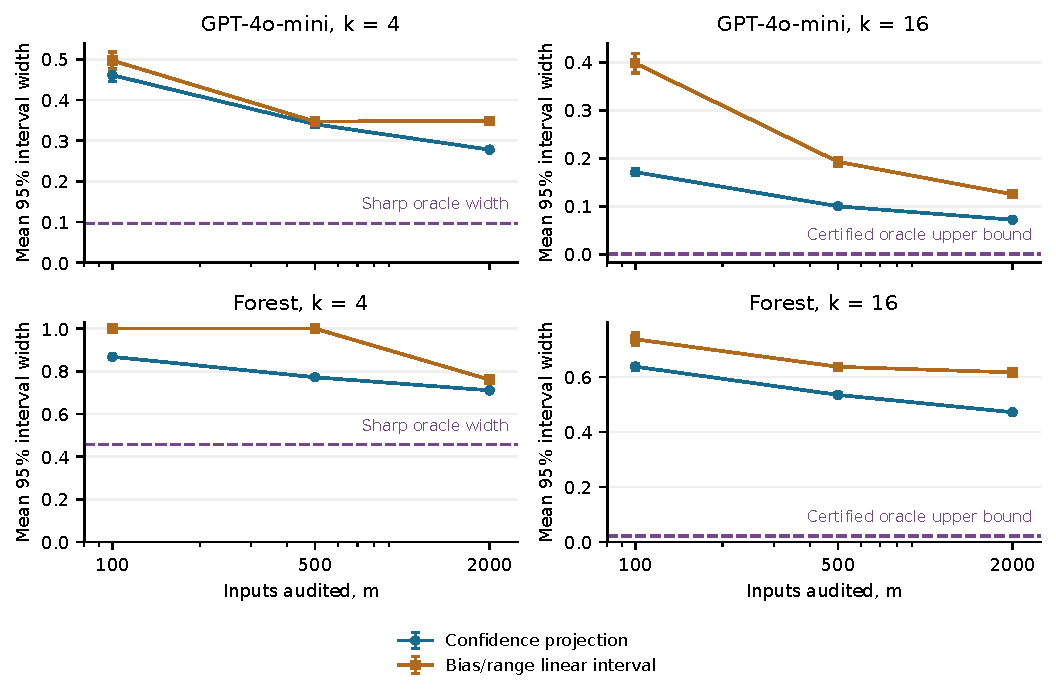
\includegraphics[width=.91\textwidth]{oracle_results/oracle_vs_finite.pdf}
\caption{Finite-sample 95\% interval width versus certified population ambiguity for two fixed populations. Error bars are $1.96$ Monte Carlo standard errors over 100 replications. The $k=4$ reference is sharp to the stated certificate tolerance; the $k=16$ reference is a certified upper bound. Width above the reference can reflect sampling uncertainty and conservatism of the chosen inference procedure.}\label{fig:oracle}
\end{figure*}

The distinction materially changes the interpretation of wide intervals. For GPT-4o-mini at $k=16$, mean projection widths at $m=100,500,2000$ are .1712, .1000, and .0719, while oracle width is at most .0002046. For Forest they are .6381, .5353, and .4722, versus at most .02159. At $m=500$, the respective mean-width standard errors are .00151 and .00363. Figure~\ref{fig:oracle} shows both depths. Thus the entire finite width cannot be attributed to nonidentification. Its excess also includes finite-sample uncertainty and inference conservatism; this experiment does not separate those two components optimally.

At classifier depth $k=64$, both population identified sets are singletons (Appendix~\ref{app:empirical-detail}), although finite-sample intervals can remain broad.

The linear baseline is narrower than projection in only two settings; Appendix~\ref{app:empirical-detail} gives coverage and risk diagnostics.

\subsection{Allocation with completion and early stopping}
The measured-population comparison fixes an available budget $B=18{,}000$ for $d=36$ and $B=19{,}600$ for $d=98$. Completion uses $k\in\{4,16\}$ and screening-budget fractions $f\in\{.25,.50,.75\}$, with
\[
 m=\lfloor fB/k\rfloor,\qquad
 R=\min\{m,\lfloor(B-mk)/(d-k)\rfloor\}.
\]
Only $f\geq k/d$ is retained, a design constraint excluding the four StrongREJECT settings with $k=16,f=.25$. The exact reserved ceiling $mk+R(d-k)$ can be slightly below $B$ because of rounding. These fixed allocations are not chosen from observed performance.

The full-label baseline fixes $\lfloor B/d\rfloor$ independent records. It and the completion design stop at the first success on each record. Count projection and the linear estimator use $\lfloor B/k\rfloor$ records with all $k$ outcomes. Detection-only inference uses the same number of records and stops after the first success or $k$ queries. Saved evaluations are not reinvested. Completion and full auditing use their unbiased estimators; the linear estimate is clipped. For the two interval-only baselines, reported point estimates are interval midpoints. Those midpoint MSEs describe explicit operational choices, not minimax estimators.

All 74 retained method/design settings use 300 independent replications, giving 22,200 trials. Figure~\ref{fig:cost} reports every allocation. Table~\ref{tab:mse} gives a fixed $f=.5$ comparison on the classifier populations, including mean-width and MSE uncertainty. Full first-success auditing uses substantially fewer actual evaluations in these settings. Completion at $k=16$ improves logistic MSE, but has a slightly wider confidence interval and more than twice the mean expenditure. For Forest, the empirical MSE difference is small relative to Monte Carlo error; exact variances are .000829 for full auditing and .000720 for completion. Point-estimation efficiency and interval precision must therefore be assessed separately.

\begin{table*}[t]
\caption{Classifier allocation comparison at available budget $B=19{,}600$ and screening fraction $f=.5$. Parentheses give one Monte Carlo standard error over 300 replications. MSE and its standard error are multiplied by $10^4$. Cost is the mean number of actually evaluated suite outcomes.}\label{tab:mse}
\centering
\begin{tabular}{llrrrr}
\toprule
Population&Method&MSE $\times10^4$&95\% interval width&Actual cost&Reserved ceiling\\
\midrule
Logistic&Full labels&3.36 (.25)&.07565 (.00048)&4,658 (23)&19,600\\
&Completion, $k=4$&4.90 (.38)&.10583 (.00081)&11,491 (19)&19,576\\
&Completion, $k=16$&2.08 (.17)&.08222 (.00048)&10,128 (21)&19,550\\
Forest&Full labels&7.24 (.58)&.11701 (.00030)&7,973 (30)&19,600\\
&Completion, $k=4$&11.29 (.97)&.17337 (.00058)&13,633 (22)&19,576\\
&Completion, $k=16$&7.10 (.59)&.15157 (.00045)&13,111 (20)&19,550\\
\bottomrule
\end{tabular}
\end{table*}

\begin{figure*}[t]
\centering
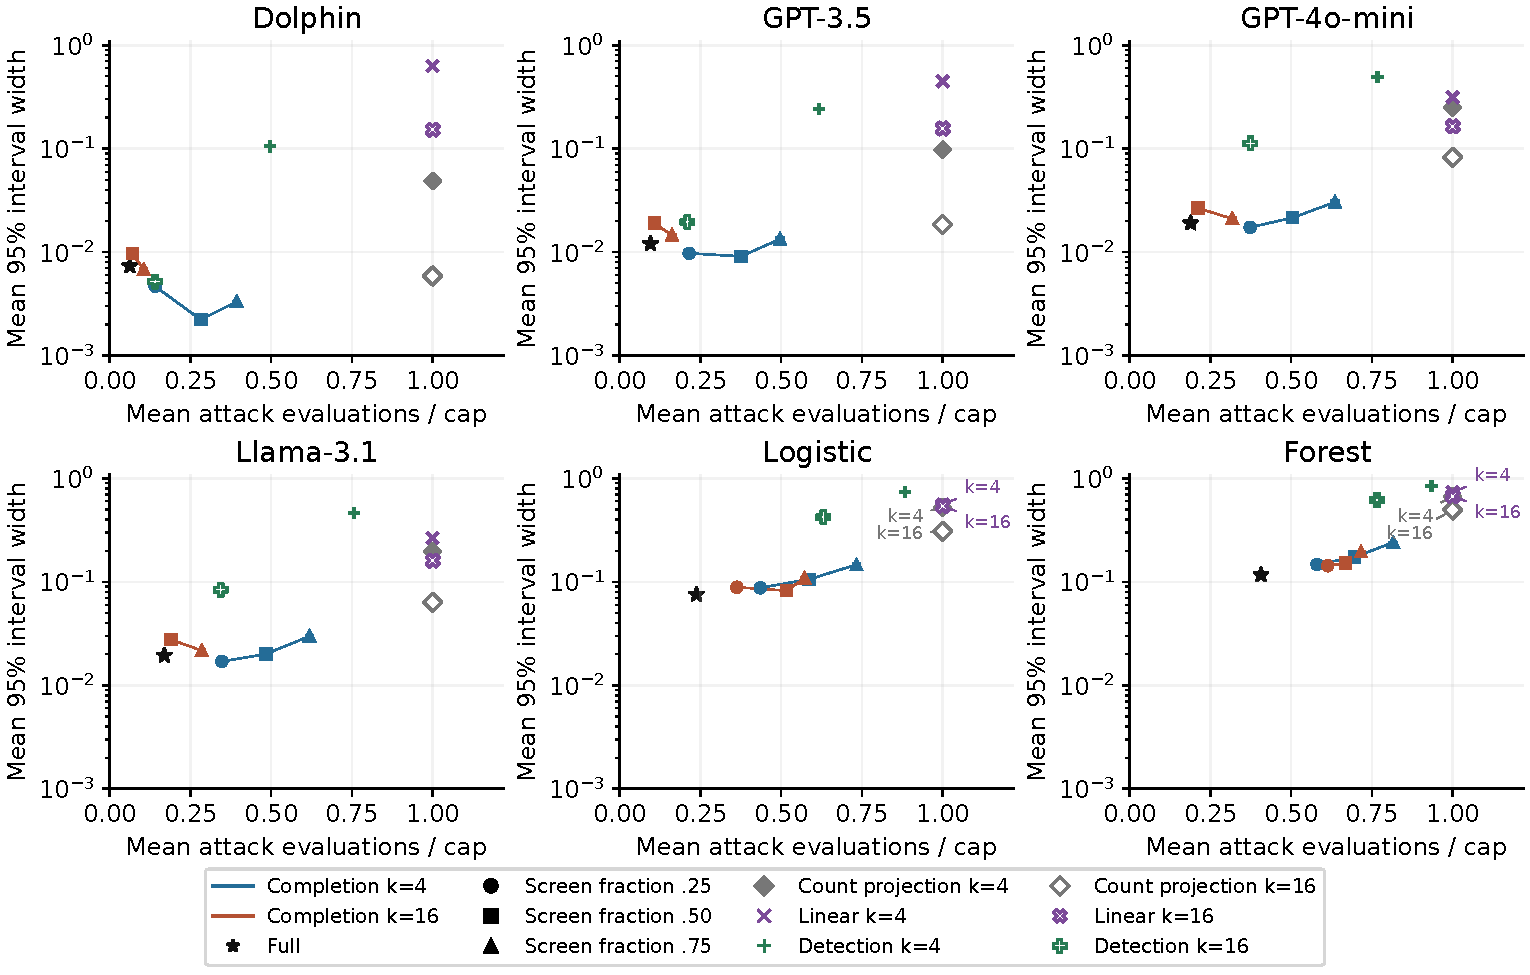
\includegraphics[width=.96\textwidth]{completion_results/main_cost_width.pdf}
\caption{Mean 95\% interval width against actual evaluations as a fraction of available budget. All retained allocations are shown; lines connect fixed screening fractions within a completion depth. Completion error bars are $1.96$ Monte Carlo standard errors and are often smaller than the symbols. The full-label comparator stops on first success, so its actual cost can be far below the reserved ceiling.}\label{fig:cost}
\end{figure*}

Full-label auditing costs only 1,125--3,401 evaluations on the nearly saturated StrongREJECT populations. Completion can nevertheless yield narrower intervals: Dolphin's $k=4,f=.5$ width is .002225 versus .007351 for full auditing, at costs 5,078 versus 1,125. Another counterexample to pointwise dominance is the original $m=500,k=16$ Dolphin projection: width .0103 versus .0165 for 222 full labels at the same reserved ceiling.

Retaining counts narrows the GPT-4o-mini and Forest intervals at $k=4$ but costs more evaluations. Dolphin at $k=16$ reverses the width ranking. Appendix~\ref{app:empirical-detail} reports these comparisons at fixed reserved ceiling and depth; they are not equal-actual-cost frontiers.

Threshold sensitivity changes the cost--precision tradeoff's magnitude (Appendix~\ref{app:empirical-detail}); it does not establish interval-ranking stability.

Measured completion coverage ranges from .9833 to 1. The guarantee rests on the conditional-binomial proof; Appendix~\ref{app:empirical-detail} reports independent numerical checks.

\subsection{Controlled prevalence and low-failure certification}
The high empirical failure rates do not directly test certification of a reliable system. A controlled study therefore retains the conditional success-count distribution $S\mid S>0$ from two specified templates, GPT-4o-mini and Forest, and changes only the zero mass. For each $\vartheta\in\{.001,.01,.05,.2,.5,.9\}$,
\[
 \mu^{(\vartheta)}_0=1-\vartheta,\qquad
 \mu^{(\vartheta)}_s=\vartheta\,\mu_s/\theta\quad(s>0).
\]
These are synthetic prevalence mixtures, not additional model measurements or estimates of deployment prevalence. Budgets are $d\times\{50,200,800\}$, with $k=4$ and $f=.5$. Five methods and 300 replications per setting give 54,000 trials.

The primary certification event is a valid one-sided 95\% upper bound at most $\tau=.05$. Full and detection methods use one-sided binomial bounds; completion splits .05 between one-sided bounds for $a$ and $b$ and maps them as in~\eqref{eq:completion-ci}. The linear method uses its bias allowance and one-sided Hoeffding radius. Projection uses its two-sided 95\% interval's upper endpoint, a conservative 95\% upper bound. A separate precision event is two-sided interval width at most .10. These constructions have different conservatism: the comparison evaluates the implemented methods, not optimal confidence procedures under each allocation.

\begin{figure*}[t]
\centering
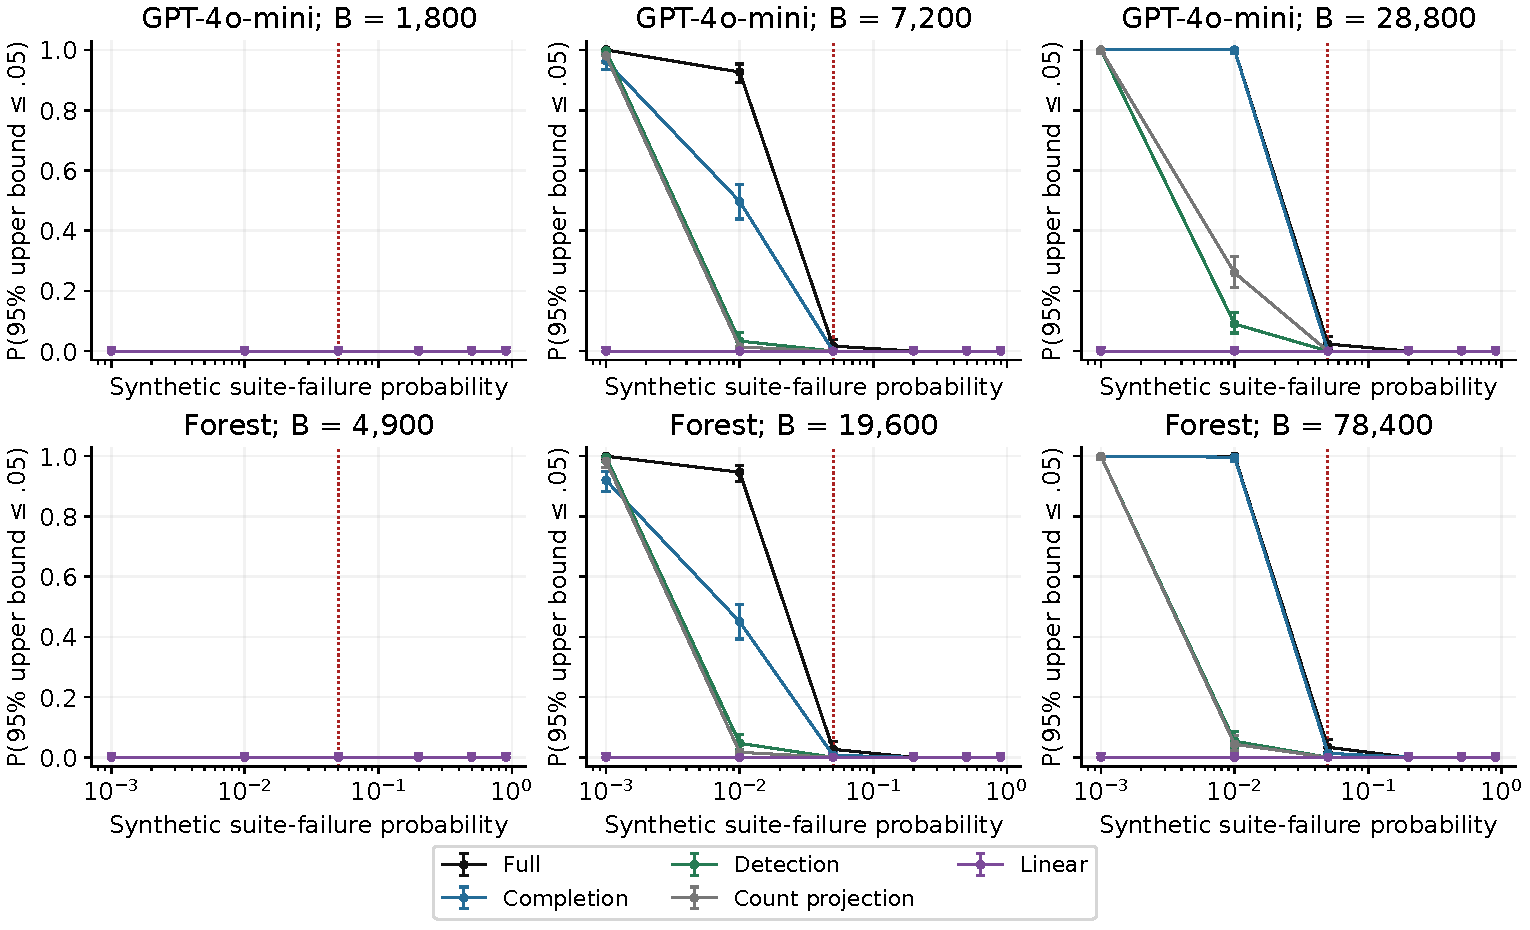
\includegraphics[width=.96\textwidth]{completion_results/controlled_certification.pdf}
\caption{Certification success for the five audit methods with their implemented confidence procedures: probability that a valid 95\% upper bound is at most .05 under synthetic prevalence mixtures. Full and detection use direct one-sided binomial bounds; completion uses two component bounds, and projection uses a two-sided interval endpoint. Vertical dotted lines mark the certification threshold. Every tested prevalence and budget is shown. Error bars are exact binomial 95\% Monte Carlo intervals over 300 replications. Lines join tested values for readability and do not assert behavior at untested prevalences.}\label{fig:certification}
\end{figure*}

Figure~\ref{fig:certification} separates point precision from the performance of the implemented upper bounds. At synthetic $\vartheta=.01$ and $B=7{,}200$ for the GPT-4o-mini template, exact full/completion variances are $4.950\times10^{-5}$ and $4.779\times10^{-5}$. Completion improves variance by 3.46\%, yet its certification probability is .4967 (95\% Monte Carlo interval [.4387,.5547]), versus .9267 ([.8911,.9535]) for full auditing. Mean two-sided widths are .05879 and .03308, respectively. Comparable point variance therefore coexists with substantially weaker certification. Variance alone does not determine tail probabilities; the comparison also depends on the sampling distributions and the two-component interval construction.

For Forest at $B=19{,}600$, exact full/completion variances are $4.950\times10^{-5}$ and $7.684\times10^{-5}$. Completion has 55.24\% higher variance, so its allocation also loses point precision. Its certification probability is .4500 ([.3928,.5082]), versus .9467 ([.9148,.9692]) for full auditing; widths are .05816 and .03296. Both designs spend nearly the available budget at these low prevalences. The globally regularized linear estimator has substantial approximation bias near this boundary and never certifies in these $\vartheta=.01$ settings. At the largest tested budgets, full auditing and completion both certify with high probability.

Appendix~\ref{app:empirical-detail} reports coverage and smallest-tested-budget results, without claiming optimized budgets.

\subsection{Learning an attack order from a separate pilot}\label{sec:ordering}
A supporting study uses one 50-record pilot per population, seed 20260923, and shared pilot contexts across the four StrongREJECT models. Revealing all pilot outcomes costs $50d$. Pilot-positive records are elements and each attack covers the records it breaks: summed first-success positions are the min-sum set-cover objective~\cite{minsumcover}; all-zero records add a constant $d$ each. The classical greedy rule covers the most uncovered records, breaking ties by coordinate index. Its factor-four pilot guarantee implies no held-out guarantee. The order is computed only from pilot outcomes and applied unchanged to held-out rows; this is not an external preregistration claim. The remaining 263 rows per security model and 644/651 classifier rows define the held-out populations.

Table~\ref{tab:ordering} shows 22.3--67.7\% lower per-record cost. On the same fixed fresh cohort, $r=B/d=500$ or 200, both orders reveal identical labels. Including the extra pilot, only GPT-4o-mini and Llama save expected expenditure: 3,490 to 3,218 and 3,111 to 2,806. Learned and uniform hard ceilings here are $B+50d$ and $B$, respectively.

\begin{table}[t]
\caption{Held-out evaluations per full label, excluding the $50d$ pilot. $n_*$ is its expected break-even cohort size on the single frozen split.}\label{tab:ordering}
\centering
\begin{tabular}{lrrr}
\toprule
Population&Uniform order&Learned order&$n_*$\\
\midrule
Dolphin&2.249&1.156&1,647\\
GPT-3.5&3.466&1.878&1,134\\
GPT-4o-mini&6.980&2.837&435\\
Llama-3.1&6.222&2.011&428\\
Logistic&23.271&12.528&457\\
Forest&39.949&31.057&552\\
\bottomrule
\end{tabular}
\end{table}

With the same \emph{end-to-end} ceiling $B$, the pilot instead leaves $r-50$ fresh records. For this held-out-only target, nonsaturated variance rises by 11.1\% or 33.3\%, and expected binomial interval widths rise in every population. Only the same two populations save total expected expenditure. Pilot labels are excluded and savings are not reinvested.

That precision penalty is specific to the separate held-out target. If pilot and follow-up records are independent draws from the same $P$, all $r$ complete labels can be pooled: their unconditional sum is $\Bin(r,\theta)$, retaining variance $\theta(1-\theta)/r$ and usual binomial inference. Learning an order does not change a complete label.

Low prevalence also limits cost gains. A positive record costs at most $(d+1)/2$ in expectation under uniform ordering and at least one under any order; a negative costs $d$ under both. Expected saving per fresh record is therefore at most $\theta(d-1)/2$. For the extra, fully charged $50d$ pilot and the same fresh cohort, nonnegative net saving for $d>1,\theta>0$ requires
\[
 n\geq\left\lceil\frac{100d}{\theta(d-1)}\right\rceil.
\]
At $\theta=.01,d=36$, this is at least 10,286 records. This optimistic necessary condition concerns the unpooled cost convention, not optimal pilot size or pooled inference. The fixed-split results do not establish deployment transfer; the artifact retains orders, paired costs, and isolation checks.

\section{Discussion}
The main consequence distinguishes reducing sampling error from obtaining the information needed for certification. Under the cap, the constructed low-rate population remains indistinguishable from one above the threshold for every fixed cohort size. Relaxing the cap permits useful certification power on that same population. This obstruction applies to every uniformly valid capped gate; the empirical ranking of completion and count procedures depends partly on the implemented bounds. The zero-detection result calibrates a narrower event and yields only a 2.3\% budget saving in the stated contract.

Breadth and restricted access are proposed policy choices, not established operational necessities. The analysis identifies when their information limits can require deeper verification; it does not recommend withholding useful features. Informative scores, unequal costs, stateful defenses, and stochastic reruns require modified analyses. Frozen replay establishes conditional behavior, not deployment risk. General confidence and expected-cost optimization lie outside these results.

\section{Conclusion}
Adaptive outcome-only hard-cap audits reduce exactly to hypergeometric mixtures. Under a total budget, complete labels plus a uniform remainder minimize worst-case zero-detection probability. The certification obstruction and supporting comparisons show why identification, precision, confidence, and expenditure must be assessed separately.

\section*{Open Science}
The accompanying artifact includes the manuscript source, analysis code, and a notebook that reproduces all reported numerical tables and figures. It also provides the measured classifier outcome matrices, audit simulation outputs, and archived JailbreakBench labels and StrongREJECT scores. The image experiment uses a bundled public dataset and requires no external model service.

\section*{LLM usage considerations}
ChatGPT and Grammarly were used for grammar and spelling checks, paraphrasing, and rewording. The assisted content was reviewed and edited, and full responsibility is accepted for the accuracy, originality, and integrity of the work.

\bibliographystyle{IEEEtran}
\bibliography{references}
\appendices
\section{Supplementary empirical comparisons}\label{app:empirical-detail}

At classifier depth $k=64$, identification is exactly a singleton. The largest observed $S$ is 55 for logistic regression and 44 for the forest. An oracle count law assigning zero probability to counts above those maxima forces the same support bound on any compatible $\mu$; the remaining moments identify that distribution. A conservative finite-sample interval can still be broad when these population equalities are not known exactly.

The population-independent linear baseline has narrower intervals than projection in only two settings and covers every target in all 100 replications per setting; the Wilson lower limit is .963. Global bias control and Hoeffding uncertainty can be costly. The artifact separates analytic raw-estimator risk from empirical clipped-estimator MSE.

Measured completion coverage ranges from .9833 to 1; the artifact retains binomial Monte Carlo intervals and risk/cost summaries. The coverage guarantee rests on the conditional-binomial proof. Independent boundary enumerations and a separate 40,000-replication check validated the formulas; simulated mean, variance, and cost agreed within .51 Monte Carlo standard errors.

A fixed sensitivity analysis rethresholds the four StrongREJECT matrices at .25, .5, and .75 and recomputes exact variance and expected stopping cost at $B=18{,}000,k=4,f=.5$. Full auditing is cheaper throughout; completion has smaller variance in every nonsaturated case. For GPT-4o-mini, completion's relative variance reduction falls from 24.31\% to 15.08\% to 1.47\%. Full/completion expected costs rise from 2,928/8,549 at threshold .25 to 4,501/10,152 at .75. The cost--precision tradeoff persists in this check, but its magnitude is sensitive to the failure definition. Threshold changes change the target, and these moment calculations do not establish confidence-interval ranking stability.

The artifact records the smallest \emph{tested} budget for which the lower 95\% Monte Carlo limit of each success probability reaches .90. For Forest at $\vartheta=.01$, that certification criterion is attained at available budgets of 19,600 for full auditing and 78,400 for completion. Both attain the width criterion at an available budget of 19,600. These are grid results, not optimized minimum budgets or claims about intermediate values. Controlled completion coverage ranges from .9800 to 1. No false certifications occur in the tested $\vartheta>.05$ cases, but zero events in 300 trials still have a positive Monte Carlo upper confidence limit.

Retaining counts can substantially narrow the interval compared with retaining detection alone. At $k=4$, GPT-4o-mini count projection has mean width .2494 versus .4954 for detection-only inference, costing 18,000 versus 13,808 evaluations; Forest gives .6708 versus .8511 at costs 19,600 versus 18,318. Dolphin at $k=16$ reverses the width ranking: .005880 for counts versus .005191 for detection, with 7.12 times the expenditure. These comparisons hold the reserved ceiling and depth fixed; they are not frontiers at equal actual cost. Extra overlap information can help, while collecting all counts and splitting the confidence error budget can make that choice unattractive near saturation.

\section{Elementary identification checks}\label{app:checks}
For the first equality, an input with one uniformly located success is indistinguishable after one query from a population that has all $d$ successes with probability $1/d$ and otherwise none. The matching upper bound uses $p(s)=s/d+(d-1)/(2d)$, whose maximum error is $(d-1)/(2d)$. For the second, the nullspace of the degree-$(d-1)$ moments is generated by $((-1)^s\binom ds)_{s=0}^d$. Its normalized positive and negative parts differ in zero mass by $2^{1-d}$. The last equality follows from observing $S$ itself.

\section{Proof of the completion result}\label{app:completion-proof}
\begin{proof}
Conditional on the full cohort and screening results, write $Z$ for the hidden positive labels among the $M$ negative screens. For $M>0$, uniform selection gives $\E[X/r]=Z/M$, so the conditional mean of~\eqref{eq:completion-estimate} is the full-cohort mean $(N+Z)/m$. For $M=0$, both means equal one. The unconditional mean is therefore $\theta$.

Conditional only on the screening indicators, the negative labels are independent Bernoulli$(b)$ variables. Thus $X\mid N\sim\Bin(\min(R,m-N),b)$, although $N$ and $X$ are not generally independent. The law of total variance gives
\[
 \frac{a(1-a)(1-b)^2}{m}
 +\frac{b(1-b)}{m^2}\E\!\left[\frac{M^2\ind\{M>0\}}{\min(R,M)}\right].
\]
The summand is defined to be zero at $M=0$. Separating $M\leq R$ and $M>R$ and using $\E M=m(1-a)$ yields~\eqref{eq:completion-variance}.

The first binomial interval misses $a$ with probability at most $\delta/2$. For every screening-indicator vector, the second misses $b$ with conditional probability at most $\delta/2$, including the $r=0$ convention. A union bound and monotonicity of $a+(1-a)b$ prove~\eqref{eq:completion-ci}.
\end{proof}

\section{Expected expenditure with early stopping}\label{app:cost}
For $s$ successes among $d$ attacks, write
\[
 q_k(s)=\frac{\binom{d-s}{k}}{\binom dk},\qquad
 t_k(s)=\sum_{j=0}^{k-1}\frac{\binom{d-s}{j}}{\binom dj}.
\]
These are the probability of a negative screen and the expected screening expenditure. Conditional on a negative screen, completing a record with $s>0$ successes requires expected additional cost $(d-k+1)/(s+1)$; for $s=0$ it requires $d-k$. Denote this function by $u_k(s)$ wherever $q_k(s)>0$. If $p=\sum_s\mu_s q_k(s)>0$, let
\[
 \gamma=p^{-1}\sum_s\mu_s q_k(s)u_k(s).
\]
Terms with $q_k(s)=0$ are defined to contribute zero. Set $\gamma=0$ for $p=0$. Since $M\sim\Bin(m,p)$ and selected negative records have the same conditional law,
\begin{equation}\label{eq:actual-cost}
 \E B_{\rm actual}=m\sum_s\mu_s t_k(s)+\E[\min(R,M)]\gamma.
\end{equation}
This expectation is used only to check the simulated expenditure. The deterministic ceiling remains~\eqref{eq:completion-budget}, and the design does not use the empirical population's unseen outcomes to choose its allocation.


\section{Data preparation and classifier details}\label{app:data}
Pixel intensities in the 1,797 handwritten digit images are divided by 16. A stratified split with seed 20260920 gives 1,078 training and 719 test images. Logistic regression uses $C=1$, L-BFGS, and at most 3,000 iterations. The forest uses 200 trees, default unrestricted depth, and seed 20260920. Neither model is tuned on audit outcomes. Only clean-correct test images are eligible; clean accuracies are $694/719$ and $701/719$. The 98-transformation matrices require 68,012 and 68,698 transformed predictions. Complete-suite failures occur on $644/694$ and $554/701$ eligible images. Mean successful-transformation counts are 8.52 and 4.62.

At the StrongREJECT score threshold .5, positive union counts are 313, 312, 310, and 310 for Dolphin, GPT-3.5-turbo, GPT-4o-mini, and Llama-3.1-70B-Instruct. At .75 they are 313, 311, 298, and 300. Threshold changes alter the operational target, especially for the latter two models. Exact source hashes, model identifiers, primary scores, threshold sensitivities, and the view including the excluded attack configuration are in the artifact. Prompts and generated responses are not needed for this analysis and are omitted.

\section{Small historical JailbreakBench example}\label{app:jbb}
The JailbreakBench artifacts~\cite{jbb,artifacts} at commit \texttt{909e68c01d94} provide complete common support for \texttt{GCG}, \texttt{JBC}, \texttt{PAIR}, and \texttt{prompt\_with\_random\_search} on four archived models. Excluding the ten behaviors in the source's Privacy category leaves 90 behaviors. The stored \texttt{jailbroken} annotation is used, without substituting the separate historical \texttt{jailbroken\_llama\_guard1} field. The derivative retains binary outcomes, identifiers, categories, and provenance. Original attack access and budgets differ, so unit matrix queries are not equal underlying API-call costs.

\begin{table}[ht]
\caption{Historical common-method suite ($d=4$, 90 source rows). Oracle intervals condition on the complete empirical reference; they are not finite-sample confidence intervals.}\label{tab:jbb}
\centering
\begin{tabular}{lccc}
\toprule
Archived model&Union&$I(H\mu)$, $k=2$&$I(H\mu)$, $k=3$\\
\midrule
GPT-3.5&.9444&[.8926,1]&[.9056,.9444]\\
GPT-4&.8444&[.8333,.9778]&[.8417,.8444]\\
Llama-2&.8889&[.8889,.9000]&[.8889,.8889]\\
Vicuna&.9444&[.9167,1]&[.9361,.9556]\\
\bottomrule
\end{tabular}
\end{table}

For Llama-2, no behavior has more than two successful methods. At $k=3$, zero mass at three observed successes forces this support restriction and the remaining moments identify the distribution. Other rows retain nontrivial ambiguity.

\end{document}
